%
We will here investigate the linear behavior of our system.
In the end we will conclude that the behavior coincides with what is found from simplified linear theory of the system.

After perturbing the system as described in \cref{sec:initRun}, most of the noise vanishes and poloidal modes start to appear.
It has not been observed that the system reaches the linear phase unless perturbed%
\footnote{This could in principle happen if the noise at machine level assembles in just the right way such that it forms a linearly unstable mode.}%
%
.
Depending on the simulation parameters, the poloidal modes will be damped to zero so that the system will return to the steady state, or they will grow and increase in amplitude.
As the perturbations are small, the dynamics in this linear phase comes purely from the linear part of the set of equations.
In other words mode, coupling between different modes are negligible.
Thus, if we were dealing with a purely linear system the growth of the modes would continue forever.
As our system is not purely linear, mode coupling will start to become important once the perturbations have grown sufficiently big.
The mix of linear and non-linear growth will eventually reach a saturated turbulence treated, which will be treated in \cref{sec:satTurb}.
We will define the linear state as:
%
\begin{enumerate}
    \item Starting once the initial perturbation has vanished and where the modes start to show a more or less exponential growth or decay.
    \item Ending at the time where any mode, which up to that point in time has been flat or damped, suddenly shows an exponential growth.
\end{enumerate}
%

\section{The linear growth}
%
In addition to the growth explained above, the modes are rotating in the linear phase.
This is indicated in \cref{fig:modeRotation}, where an clockwise rotation is observed.
For further reference, one should note that the black dashed circles on the perpendicular part of the plot indicates the position of the maximum gradient of the density in the steady state, which is also the fixed $\rho$ in the poloidal part of the plot.

We will now compare the direction of rotation of the perturbations with direction of rotation of the zeroth order drifts.
In \cref{fig:modeRotation} the magnetic field is pointing into the paper.
Further, the gradient in both $\phi$ and $n$ is point towards the center (i.e. towards negative $\rho$).
From \cref{poi:cylExB} have that
%
\begin{align*}
    u_{E,\theta} =& \ve{u}_{E}\cdot\hat{\ve{e}}_\theta
    %
    =
     \frac{1}{JB}
           \L(
           - \ve{e}_\theta\partial_\rho
           + \ve{e}_\rho\partial_\theta
           \R)
           \phi
    \cdot
    \frac{\ve{e}_\theta}{\rho}
    %
    =
     - \frac{1}{J\rho B} g_{\theta\theta} \partial_\rho \phi
    %
    =
     - \frac{\rho^2}{\rho^2 B} \partial_\rho \phi
    %
    =
     - \frac{1}{B} \partial_\rho \phi,
\end{align*}
%
so the $\ve{u}_E$-drift is moving in the counter-clockwise direction%
\footnote{
Note that the signs comes as a consequence of working in a left handed system.
This means that $\theta$ is increasing in the counter-clockwise direction.
}
%
.
Substituting $\grad\phi$ with $\frac{T_e\grad n}{q_en}$ in \cref{poi:cylExB} gives the electron diamagnetic drift.
We find that
%
\begin{align*}
 u_{d,e,\theta}= \frac{T_e}{eB} \frac{\partial_\rho}{n}.
\end{align*}
%
That is, the diamagnetic drift is moving in the clockwise direction, opposite of the $\ve{E}\times\ve{B}$-drift direction.
In absolute numbers, the $\ve{E}\times\ve{B}$-drift is approximately one order smaller than the diamagnetic drift at the position of maximum density gradient for our parameters.
Hence, the perturbations are moving in the electron diamagnetic direction.
This is one of the characteristic features of drift waves \cite{Jassby1972}.
To verify if the linear phase can be identified as drift waves, we will proceed with a quick review of linear drift waves.

%
{
% FIXME: Move this figure and uncomment clearpage and thispage empty when document is done
% \clearpage
% \thispagestyle{empty}
\begin{figure}[htbp]
    \vspace*{-1cm}
    \centering
    \begin{subfigure}[h]{1.00\textwidth}
        \centering
        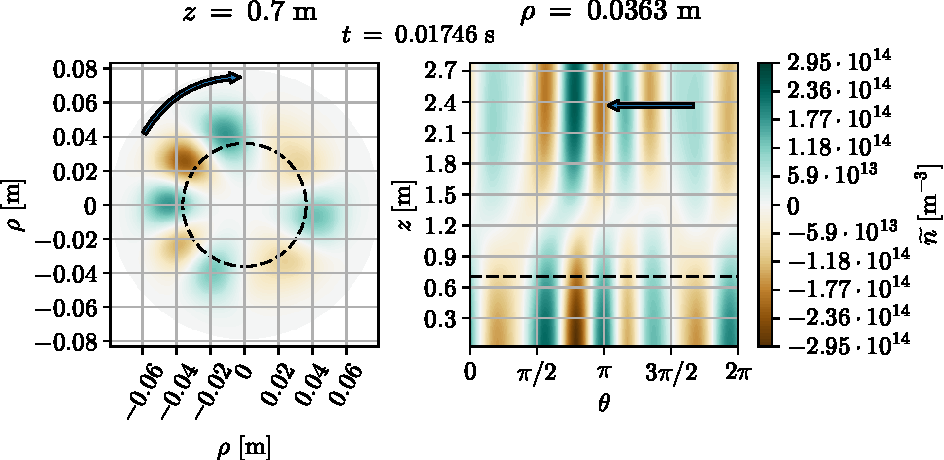
\includegraphics{fig/results/rotModes/n-perpPol-2D-fluct-0_rot}
        \label{fig:rot1}
    \end{subfigure}%
    \\
    \begin{subfigure}[h]{1.00\textwidth}
        \centering
        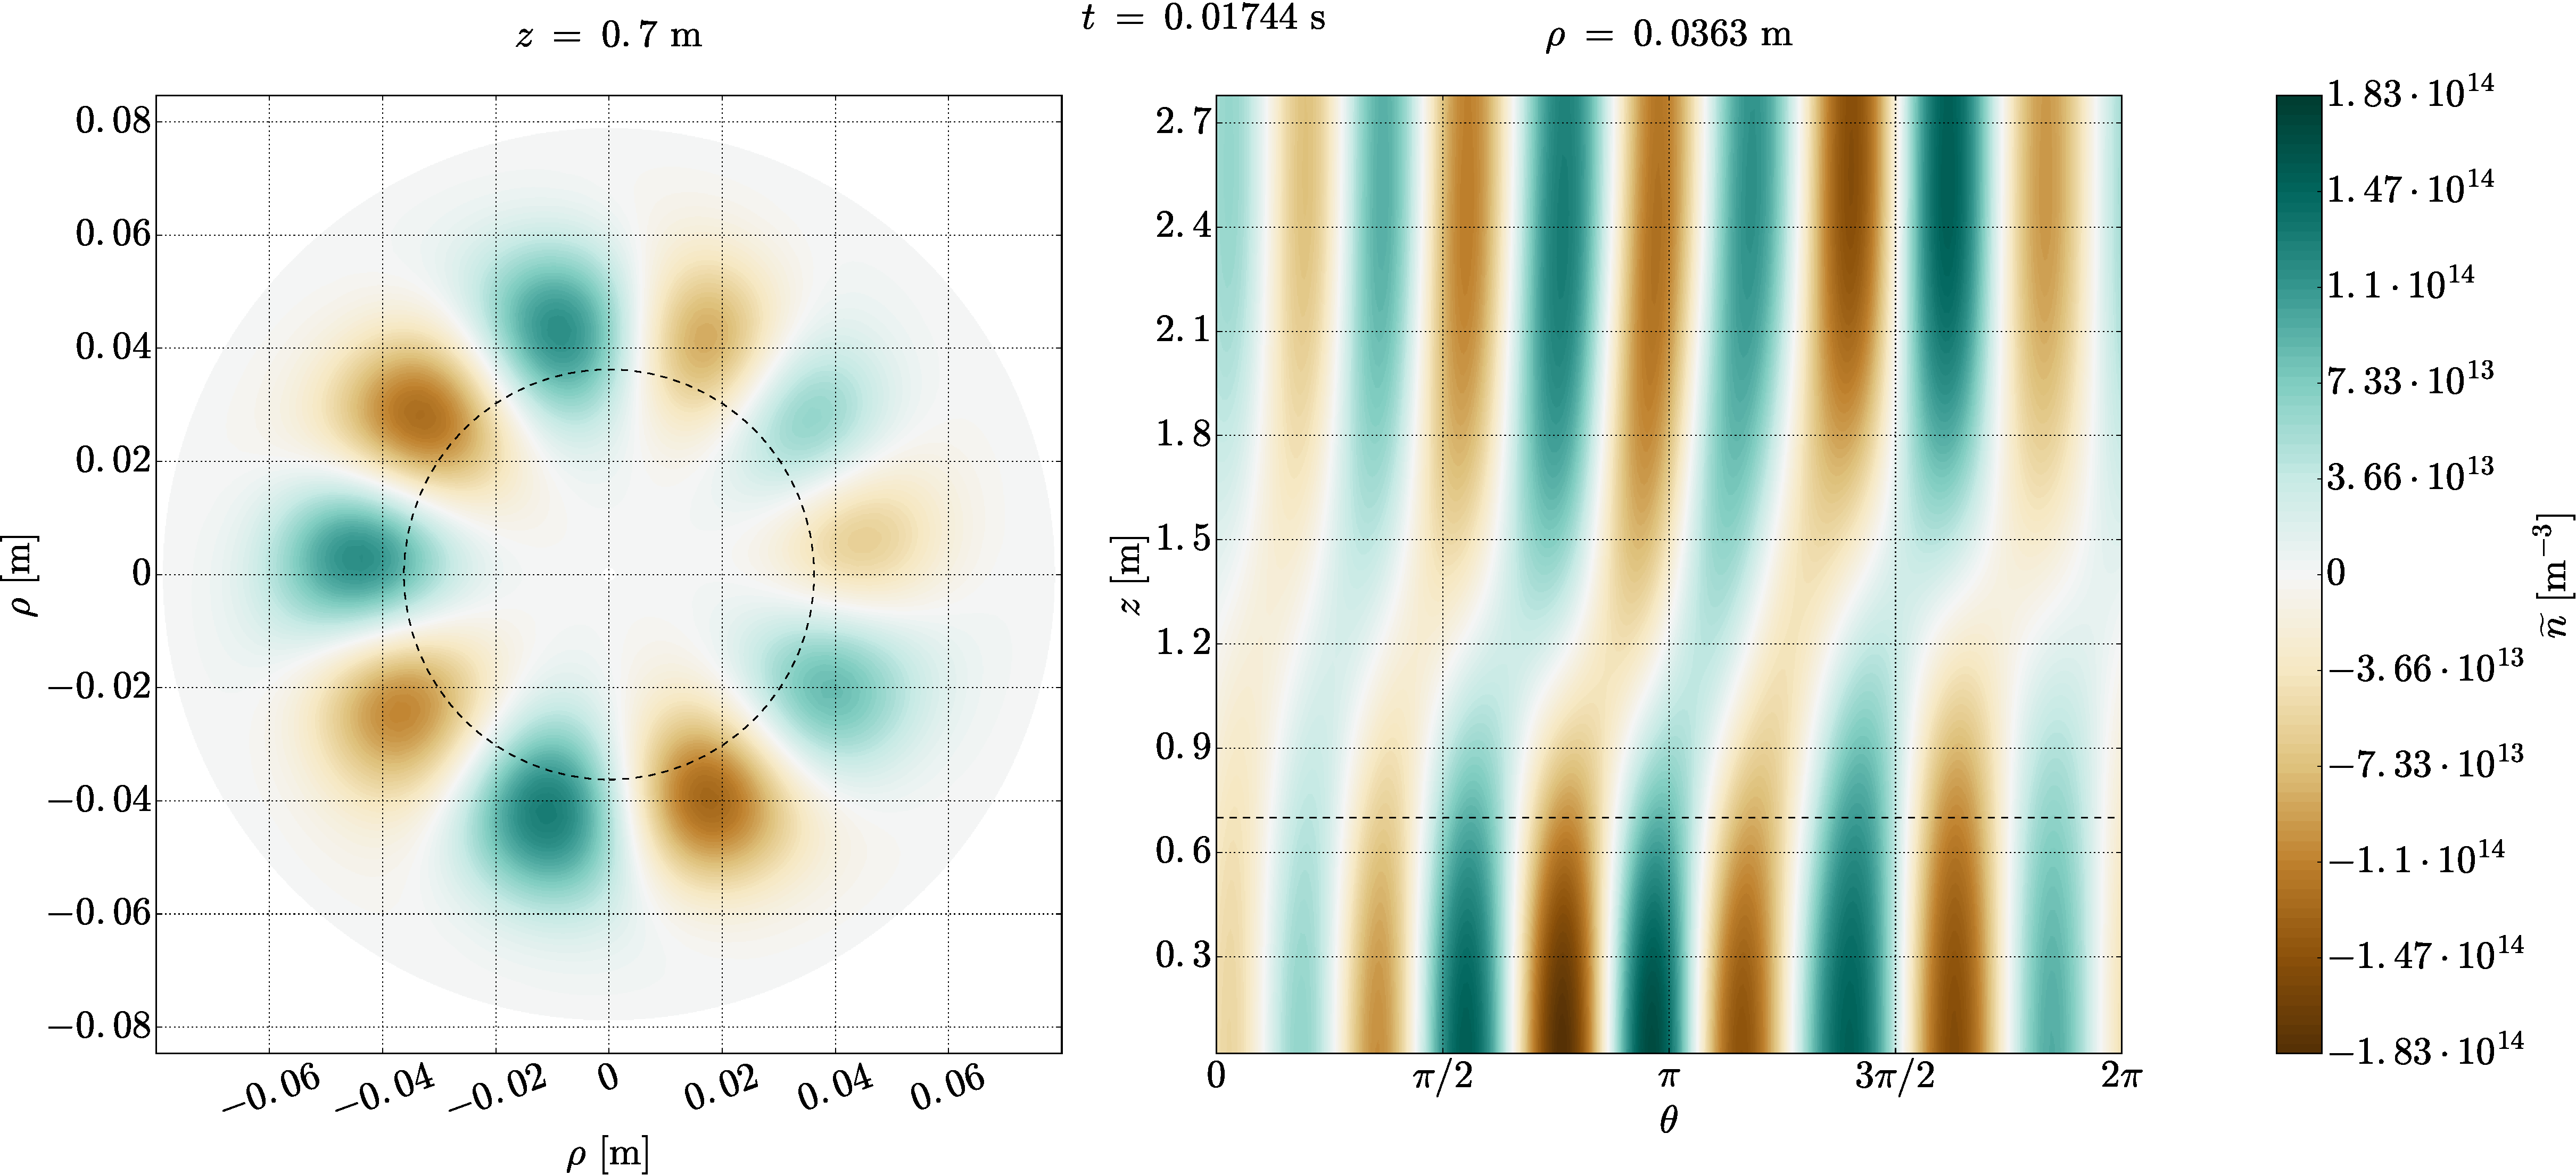
\includegraphics{fig/results/rotModes/n-perpPol-2D-fluct-1}
        \label{fig:rot2}
    \end{subfigure}
    \\
    \begin{subfigure}[h]{1.00\textwidth}
        \centering
        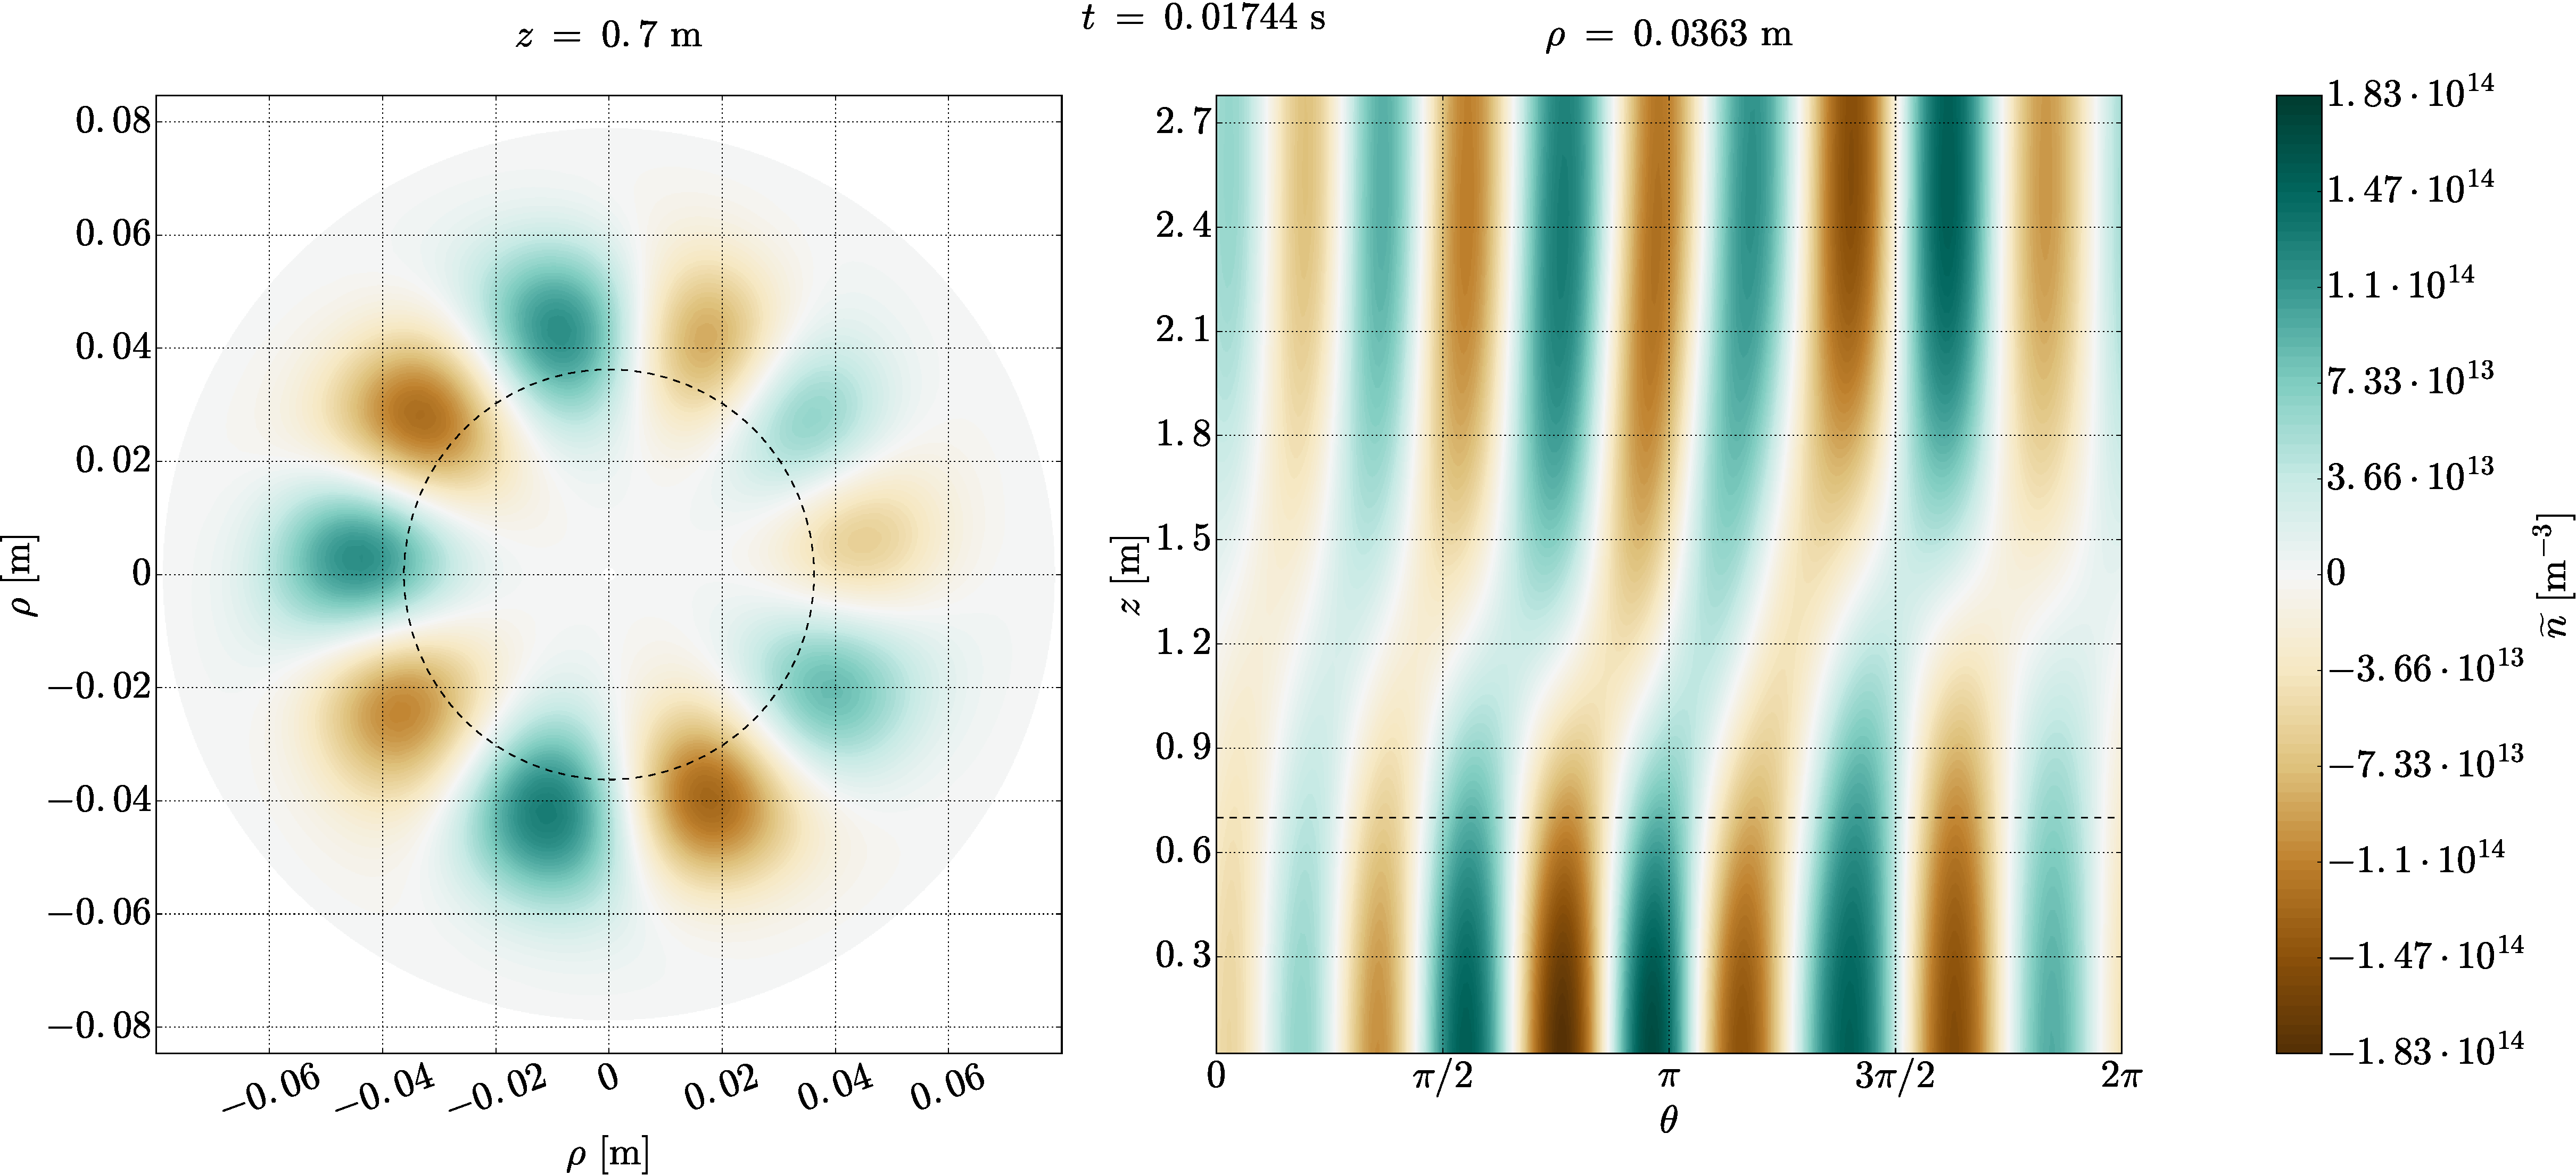
\includegraphics{fig/results/rotModes/n-perpPol-2D-fluct-2}
        \label{fig:rot3}
    \end{subfigure}
    \caption{Rotation of the modes.
        The arrow indicates the direction of movements, whilst the dashed lines indicates where the data is sliced for the opposite plot.
    }
    \label{fig:modeRotation}
\end{figure}
% \clearpage
}
%

\section{Simplified linear drift wave theory}
\label{sec:simpleLin}
%
Conceptually, a drift wave is a wave which travels in the electron diamagnetic direction, and arises due to the mass difference between electrons and ions.
If one introduce a density (or pressure) perturbation in a homogeneous, magnetized plasma in a slab, the  electrons will stream out of the perturbation along the magnetic field lines at a much faster rate than ions due to their higher mobility.
This gives rise to a $\ve{E}$-field perturbation pointing in the direction of the electrons.
The $\ve{E}$-field gives in turn rise to a $\ve{E}\times\ve{B}$-drift perpendicular to the magnetic field.
This process is depicted in \cref{fig:DW}.
%
\begin{figure}[htb]
    \centering
    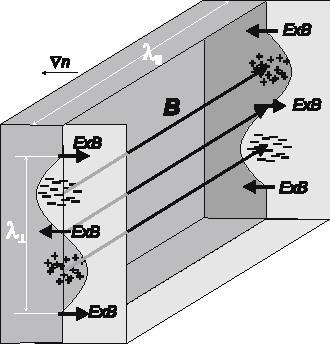
\includegraphics{fig/driftwave}
    \caption{
        Sketch of a drift wave in a slab.
        The $\ve{E}\times\ve{B}$ arrows indicates the position of the maximum $\ve{E}\times\ve{B}$-drift.
        Taken from \cite{Stroth2011book}.
    }
    \label{fig:DW}
\end{figure}
%
The drift waves has its counterpart in fluid dynamics as Rossby waves, where the $\ve{E}\times\ve{B}$ drift equivalence comes from the Coriolis force \cite{Shepherd1987}.

A phase shift is necessary in order to get an instability.
This can be seen from \cref{fig:DW} if one shifts the ion and electron clouds upwards or downwards so that the $\ve{E}\times\ve{B}$ arrows are shifted with respect to the density perturbations.
For a mathematical demonstration of this, see for example \cite{Garcia2001a}.
A phase shift arises if the parallel motion of electrons arising from pressure gradients is delayed.
Such a delay can have its origin in for example magnetic induction, Landau damping, or as in our case, due to resistivity.

To obtain a simple analytic expression of the drift waves, we will recite the most important points given in the derivation in \cite{Pecseli2016book}.
We are here not concerned with neutral interaction.
For an analytic expression where the neutral elastic collision dominates, see \cite{Ellis1980}.

The derivation in \cite{Pecseli2016book} is done by considering a magnetized plasma in Cartesian with the assumptions of:
%
\begin{itemize}[noitemsep]
    \item Cold ions.
    \item Isothermal electrons.
    \item Electrostatic conditions.
    \item No electron inertia.
    \item Quasi-neutrality.
    \item $n$ has only a gradient along $x$, where $B$ is in the direction of $z$.
\end{itemize}
%
The electron and ion momentum equations are linearized together with the electron and ion continuity equations.
No background electric field is assumed.
Perturbation of $n$, $u_e$ and $\phi$ are assumed to be on the form $A\exp\L(i[k_x x + k_y y - \L(i\Im[\om] + \Re[\om]\R) t]\R)$, where $A \in \{n, u_e, \phi\}$.
One can assure oneself that positive $\Im(\om)$ causes exponential growth for increasing $t$, and a positive $\Re(\om)$ causes the perturbation to move along $y$ as the inverse wavelength $k_y$ stays constant.
After solving the system algebraically, one arrives at the equation
%
\begin{align}
    \partial_x^2 \phi(x) +
    \frac{\partial_x n_0(x)}{n_0(x)}\partial_x \phi(x)+
    \L(k_y^2 +
    \frac{\om_{ci}}{\om}\frac{\partial_x n_0(x)}{n_0(x)}k_y -
    \frac{\om^*+ib\sigma_\|}{\om+ib\sigma_\|}\frac{\om_{ci}^2}{c_s^2}
    \R)\phi(x)
    =0,
    \label{eq:fullDisp}
\end{align}
%
where $\om^*$ is the diamagnetic frequency, $\sigma_\|$ describes the conductivity in the system and $b$ measures the extent of the perturbation compared to $\rho_s$.
These quantities are defined as
%
\begin{align*}
    \om^* \defined& k_y u_{De} =
    -\L(k_y \frac{T_e}{eB}\frac{\grad n(x)\times \ve{b}}{n(x)}\R)\ve{e}_y
    =
    k_y \frac{T_e}{eB}\frac{\partial_x n(x)}{n(x)}
    \note{Left handed coordinate system}
    \\
    %
    %
    \sigma_\| \defined& \L(\frac{k_z}{k_y}\R)^2 \frac{\om_{ce}}{\nu_{ei}}\om_{ci}\\
    b \defined& (k_y \rho_s)^2&
\end{align*}
%
\Cref{eq:fullDisp} can be solved as a second order boundary value problem by properly defining the boundary conditions.
However, an analytical solution is sought, so the approximation $\partial_x^2 \phi(x)\simeq\partial \phi(x)\simeq0$ is used.
This is essentially is a statement that the perturbations are infinite long in the $x$-direction.
The final analytic dispersion relation now reads
%
\begin{align}
    \om^2+i\sigma_\|\L(\om\L[1+b\R]-\om^*\R) = 0,
    \label{eq:analyticDisp}
\end{align}
%
where the following solution gives the maximum growth rate
%
\begin{align*}
    \Im(\om) =& - \frac{b \sigma}{2}
    \\&
    - \frac{\sqrt{\sigma}}{2}
    \L(16 [\om^{*}]^{2} + \sigma^{2} \L[b^{2} + 2 b + 1\R]^{2}\R)^{1/4}
    \\&\quad
    \sin\L(\frac{1}{2} \atan2\L[4 \om^{*},- \sigma \L(b^{2} + 2 b + 1\R) \R] \R)
    \\&
    - \frac{\sigma}{2}
    \numberthis
    \label{eq:grIm}
    \\
    %
    \Re(\om) =& - \frac{\sqrt{\sigma}}{2}
    \L(16 [\om^{*}]^{2} + \sigma^{2} \L[b^{2} + 2 b + 1\R]^{2}\R)^{1/4}
    \cos\L(\frac{1}{2} \atan2\L[4 \om^{*},- \sigma \L(b^{2} + 2 b + 1\R) \R] \R)
\end{align*}
%
We note that the maximum growth (the highest positive $\Im(\om)$) in \cref{eq:grIm} is obtained where $\om^{*}$ has a maximum, which corresponds to the position of the minimum in $\partial_x n/n$.
Analytical expression for the dispersion relation in cylinder geometry is not easy obtainable as a Fourier decomposition in the radial direction will not make sense due to the lack of periodicity in $\rho$. Despite this, analytic expression can still be obtainable by decomposition into Bessel functions, as done in a similar system in \cite{Rasmussen2006a}.
As we would like to compare the analytic growth rates with what is found from the simulations, we will use \cref{eq:analyticDisp} in slab coordinates as a comparison.
In slab coordinates we let
%
\begin{align*}
    &x \to \rho&
    &y \to \rho\theta.
\end{align*}
%
The wavenumber in the $y$-direction, can in cylindrical coordinates be approximated as
%
\begin{align*}
    k_y \simeq k_\theta
    = \frac{2\pi}{\lambda_\theta}
    = \frac{2\pi}{\frac{2\pi \rho}{m_\theta}}
    = \frac{m_\theta}{\rho}.
\end{align*}
%
Some important differences in the dispersion relations when using the slab approximation for a cylinder geometry is given in \cite{Ellis1980}.
This includes discrepancies in the trends for the critical $B$-field needed for the onset of instability, and the trend of how the instability scales with mode numbers.
These discrepancies arises from how $\rho$ enters the differential operators in cylindrical geometry, and how the wavelength changes due to the curvature of the circle.
From this, we see that the slab approximation becomes better for higher mode numbers $m_\theta$, as short wave lengths "sees" the curvature less than for long wave lengths.

\section{Analytical dispersion relation}
\label{sec:analDisp}
%
A visualization of the dispersion in slab geometry is given in \cref{eq:analyticDisp}.
Here, the value of $\partial_\rho n/n$ is taken from the steady state from the simulations.
$k_z$ is set to $\pi/L_z$, as  $\lambda_z \simeq 2L_z$, which can be observed in \cref{fig:modeRotation,fig:dominatingMode}.
In our simulation, this wavelength is a consequence of the Neumann boundary condition on the density in both ends of the cylinder.
Note that this wave length is not necessarily unrealistic, and that $k_z$ may be much larger than the machine length as explained in \cite{Chen1965}.
Finally, in order to correct for $\partial_\rho\phi$ which is absent in the analytical derivation (i.e. with no poloidal $\ve{E}\times\ve{B}$-drift), but present in the simulation, $u_{E,\theta}/\rho_{\max|\partial_\rho n/n|}$ has been added to $\Re(\om)$ in order to correct for this.
%
\begin{figure}[htb]
    \centering
    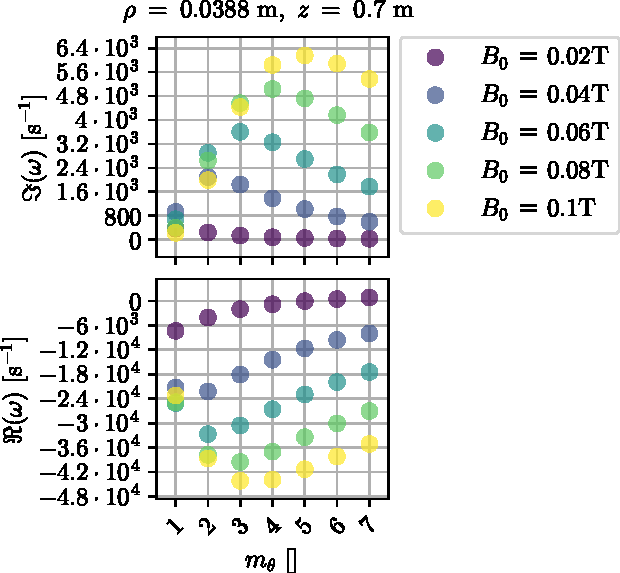
\includegraphics{fig/results/growthRates/growthRatesAnalyticB0}
    \caption{Growth rates and angular velocity as a function of mode number.
        Obtained from \cref{eq:analyticDisp}.}
    \label{fig:grAnalytic}
\end{figure}
%

In \cref{fig:grAnalytic} we can observe that the mode of maximum of the growth rates is increasing with increasing $B$.
This is also shown in \cref{fig:dominatingMode}, where one can also observe that the parallel node moves downward with decreasing $B$.
The same trend is observed for the angular frequency in \cref{fig:grAnalytic}, but here the maximum is shifted to one mode number lower as compared to the growth rates.
%
{
% FIXME: Move this figure and uncomment clearpage and thispage empty when document is done
% \clearpage
% \thispagestyle{empty}
\begin{figure}[htbp]
    \vspace*{-1cm}
    \centering
    \begin{subfigure}[h]{1.00\textwidth}
        \centering
        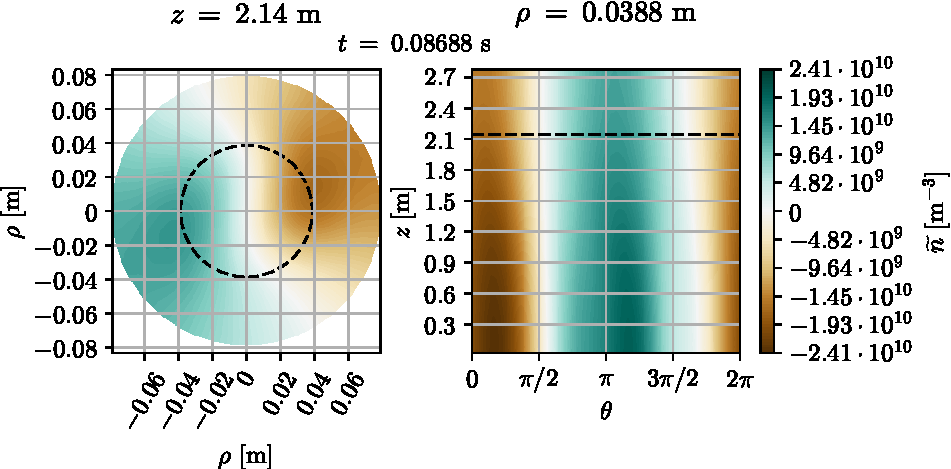
\includegraphics{fig/results/modesDiffScanVals/B002}
        \caption{$B=0.02 \T$}
        \label{fig:B002}
    \end{subfigure}%
    \\
    \begin{subfigure}[h]{1.00\textwidth}
        \centering
        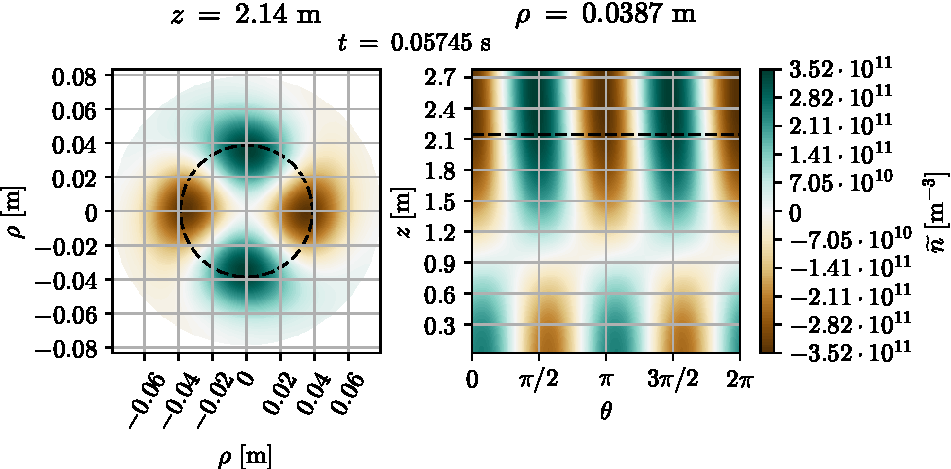
\includegraphics{fig/results/modesDiffScanVals/B004}
        \caption{$B=0.04 \T$}
        \label{fig:B004}
    \end{subfigure}
    \\
    \begin{subfigure}[h]{1.00\textwidth}
        \centering
        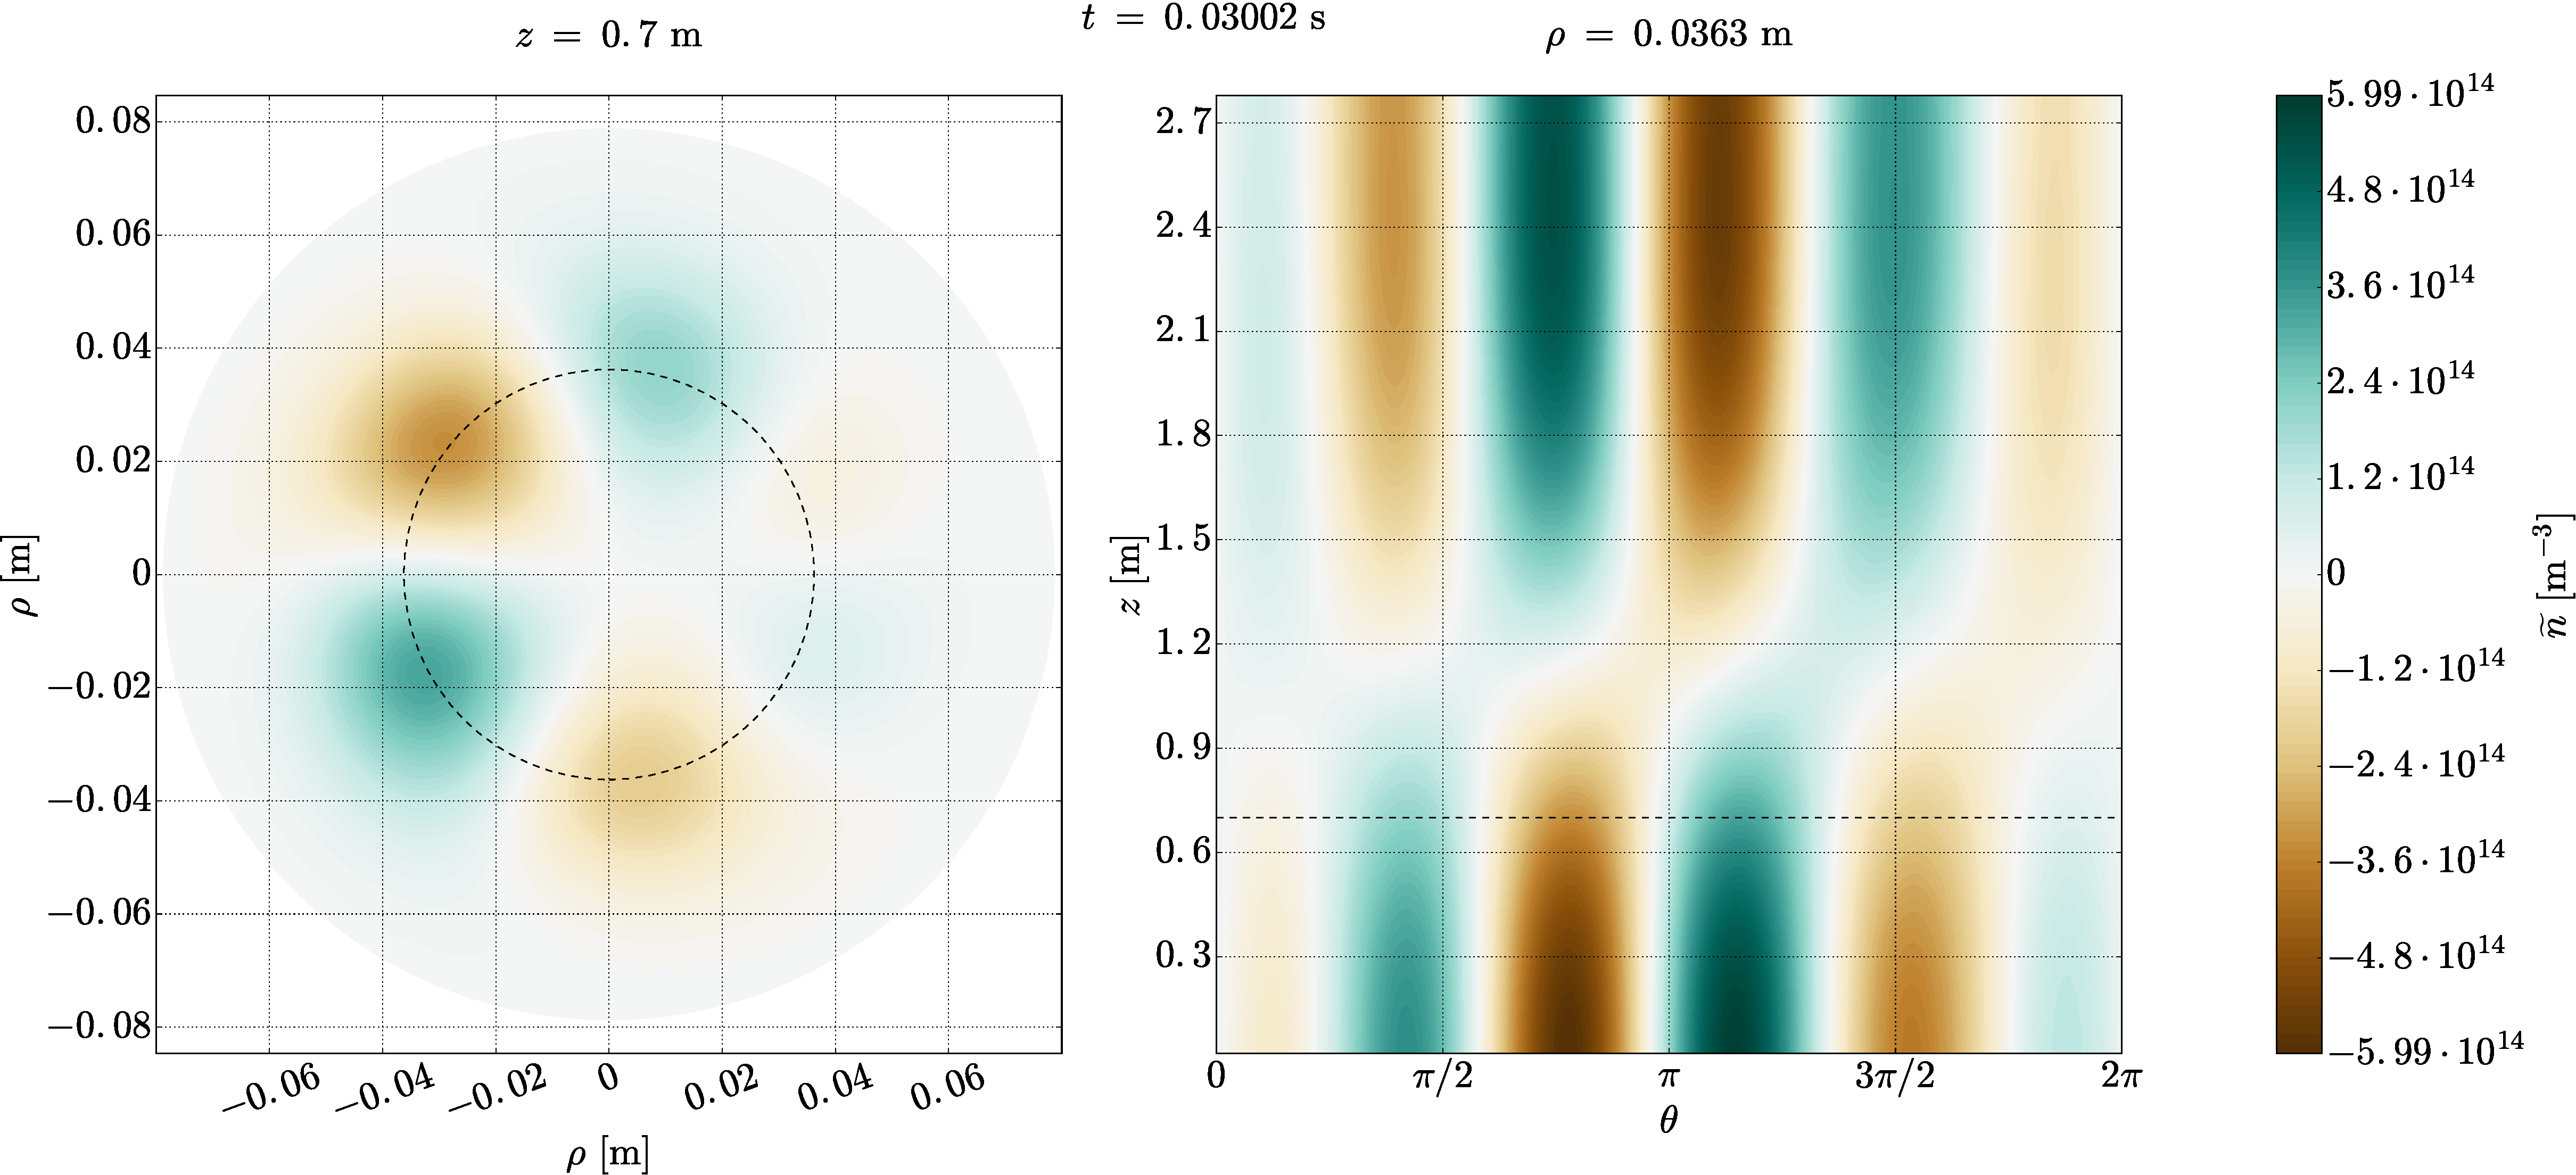
\includegraphics{fig/results/modesDiffScanVals/B006}
        \caption{$B=0.06 \T$}
        \label{fig:B006}
    \end{subfigure}
    \caption{Dominant mode depends on $B$}
    \label{fig:dominatingMode}
\end{figure}
% \clearpage
}
%

The same information as given in \cref{fig:grAnalytic} is presented in a different way in \cref{fig:grAnalyticBModeNr}.
%
\begin{figure}[htb]
   \centering
   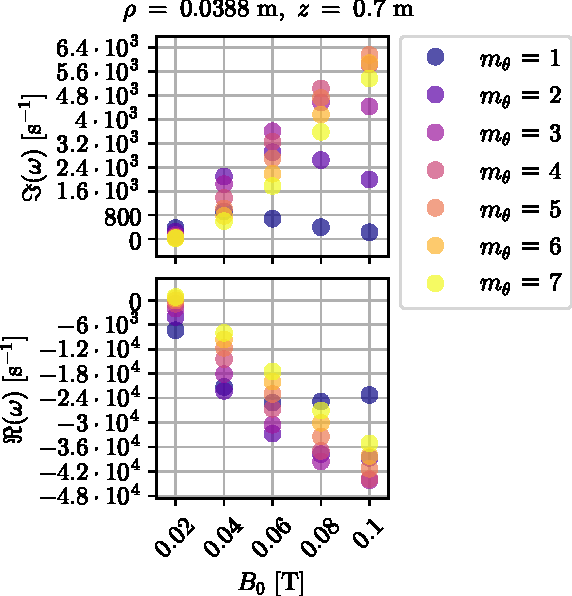
\includegraphics{fig/results/growthRates/growthRatesAnalyticB0ModeNr}
    \caption{Growth rates and angular velocity as a function of $B_0$.
        Obtained from \cref{eq:analyticDisp}.}
   \label{fig:grAnalyticBModeNr}
\end{figure}
%
From \cref{fig:grAnalyticBModeNr} we see that the growth rates of all modes are monotonically increasing with increasing $B_0$ (with an exception of $m_\theta=1$).
We can also observe that the angular frequency increases with increasing $B_0$.
This might come as a surprise, as simpler models for the drift wave predicts that $\Re(\om)\propto \om^* \propto 1/B$.
This is true also for \cref{eq:analyticDisp} in the limit of large $\sigma_\|/\om^*$ and small $b$, as pointed out in \cite{Pecseli2016book}.
However, as shown in \cref{tb:typicalLinValsB,tb:typicalLinVals} this limit is not valid in our case, and $\Re(\om)\propto B$ is observed instead.
%
\begin{table}[h!]
{\footnotesize \centerline{
\colorme
\begin{tabular}{c|cc}
\hline\hline
%
% NOTE: Lazy formatting here
Variable & Values for $m_\theta = 4$ & $B_0$-dependency \\
 & in the range $B_0=0.1\to0.02\T$&  \\
%
\hline
%
$\om^*$     & $\sim -1\cdot 10^5\s^{-1}$  & $1/B$\\
$b$         & $1\to27$  & $1/B^2$\\
$\sigma_\|$ & $6000\to275\s^{-1}$  & $B^2$\\
%
\hline\hline
\end{tabular}
}}
\caption{Values for $\om^*$, $b$ and $\sigma_\|$ for $B_0=0.1\to0.02\T$ and $m_\theta=4$.}
\label{tb:typicalLinValsB}
\end{table}
%
\begin{table}[h!]
{\footnotesize \centerline{
\colorme
\begin{tabular}{c|c}
\hline\hline
%
Variable & Values in the range $B_0=0.1\to0.02\T$ \\
%
\hline
%
$\rho_{\max|\partial_\rho n/n|}$ & $\simeq 0.037\m$\\
$\partial_\rho n/n$ & $-38 \to - 9\m^{-1}$\\
$u_{E,\theta}$ & $50-125$\\
%
\hline\hline
\end{tabular}
}}
\caption{Typical values for $B_0=0.1\to0.02\T$.}
\label{tb:typicalLinVals}
\end{table}

\section{Dispersion relation from the simulations}
%
A dispersion relation like the one found in \cref{sec:analDisp} can also be obtained from the numerical simulations.
From the individual time traces of the Fourier transformed modes of for example $n$, the growth rates can be extracted from the slope of the logarithm of the absolute value of the Fourier modes in the linear phase.
The angular frequency can be found from
%
\begin{align*}
    \Re[\om_n(t)] =
    \frac{1}{T}\sum_{i=0}^{T-1}
    \frac{
        \atan2\L(\Im[\text{FT}(n[t_{i+1}])], \Re[\text{FT}(n[t_{i+1}])]\R) -
        \atan2\L(\Im[\text{FT}(n[t_{i}])], \Re[\text{FT}(n[t_{i}])]\R)
    }{\Delta t},
\end{align*}
%
where $T$ denotes the total number of time samples in the linear phase, and $i=0$ denotes the first time point in the linear phase.

The time trace of the $7$ first modes is depicted in \cref{fig:fourierUnstable}.
%
\begin{figure}[h!]
    \centering
    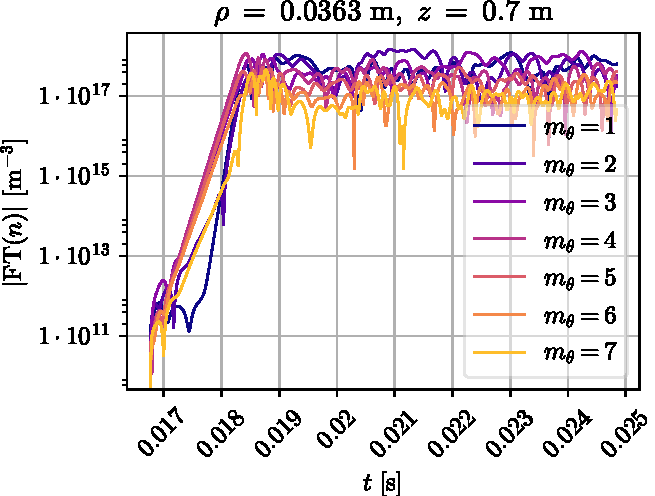
\includegraphics{fig/results/fourierModes/unstable}
    \label{fig:fourierUnstable}
    \caption{Growth rate leading to saturated turbulence for $B=0.1\T$.}
\end{figure}
%
As the ordinate in \cref{fig:fourierDens} is logarithmic, exponential grow will appear as straight lines.
One should note, that contrary to what was found in \cref{sec:analDisp}, $B=0.02\T$ shows a decaying behavior in \cref{fig:fourierStable}.
%
\begin{figure}[h!]
    \centering
    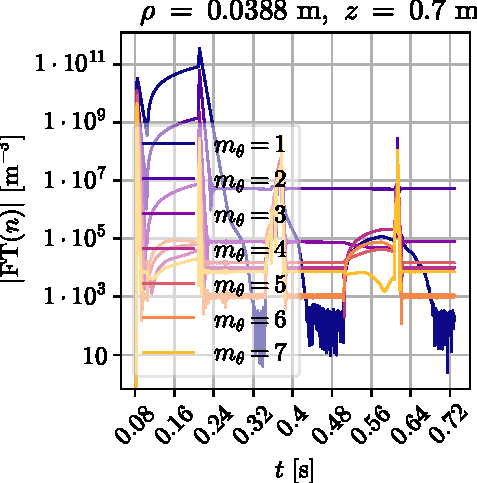
\includegraphics{fig/results/fourierModes/stable}
    \label{fig:fourierStable}
    \caption{For $B=0.02\T$ the system is stable against perturbation.}
\end{figure}
%
This can be explained by the viscosities, which is present in our model, but not accounted for in the derivation of the dispersion relation in \cref{sec:simpleLin}.
The dispersion obtained from the simulations as a function of mode number is found in \cref{fig:grB}, where the error bars in the growth rates shows the spread in the linear fit, whereas the error bar in the angular frequency represents the standard-deviation.
%
\begin{figure}[htb]
        \centering
        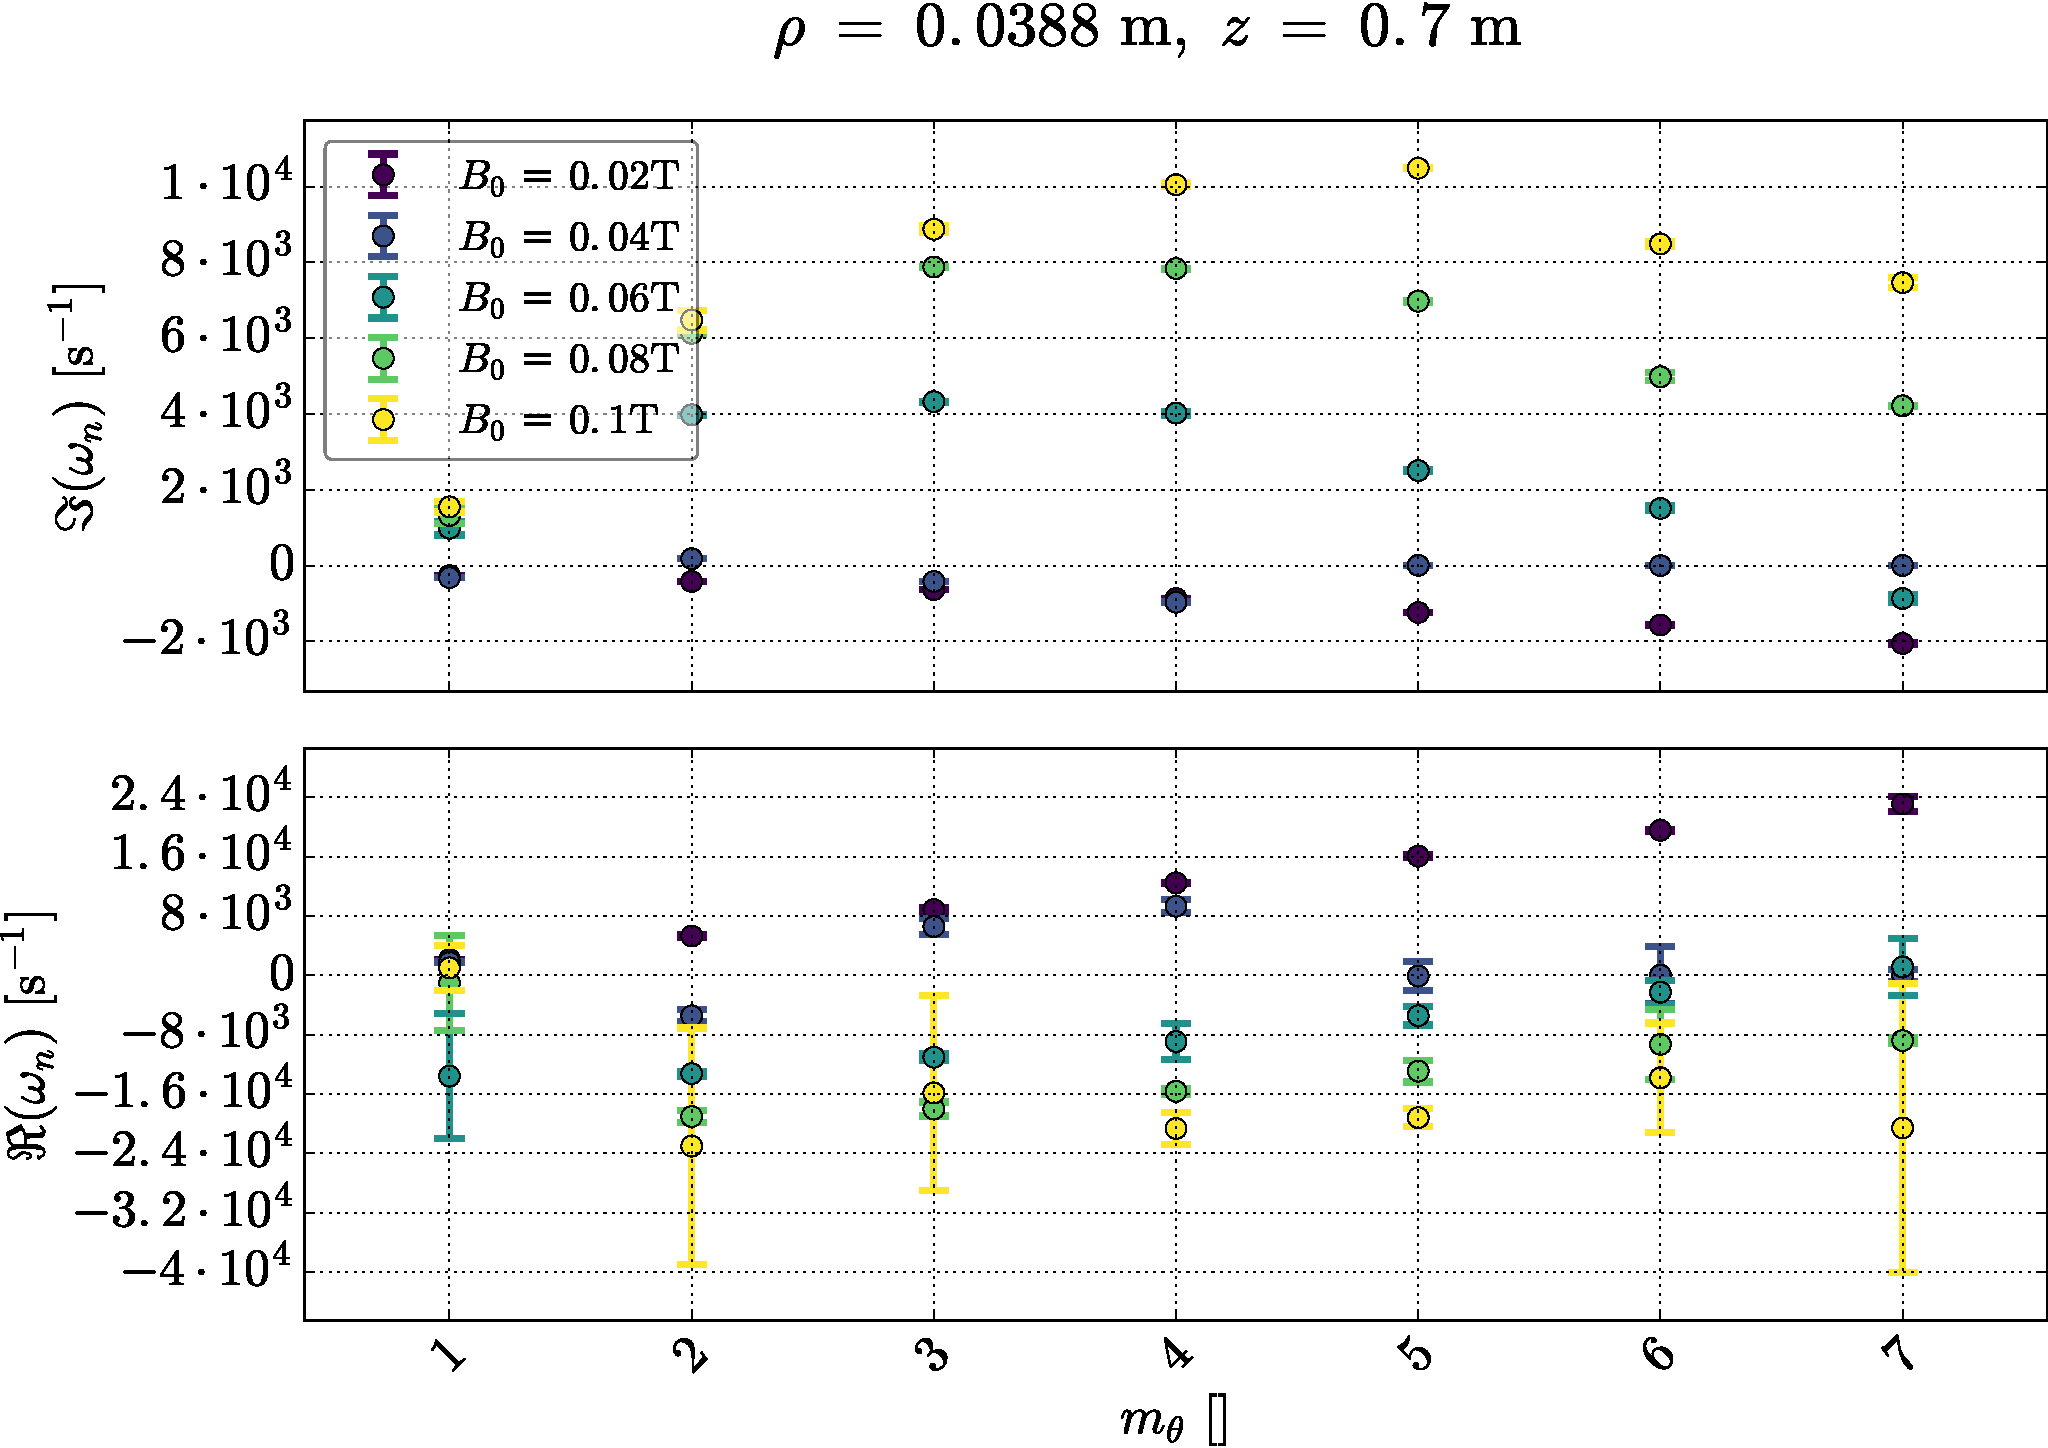
\includegraphics{fig/results/growthRates/growthRatesB0}
        \caption{Mode number-dependency on the growth rates and angular velocities.
            Obtained from the simulations.}
        \label{fig:grB}
\end{figure}
%
Both the trend and the values in \cref{fig:grB} matches approximately what was found in \cref{fig:grAnalytic}.
The maximum growth rate is shifted to one higher mode number for all $B$-field amplitudes in the growth rates found in the simulations.
For lower values of $B_0$ the growth rates found in the simulation is less than what was found in the analytical expression, which means that the growth rates for all mode number is negative for $B_0=0.02\T$.
Likewise, the angular frequency is shifted upwards for lower values of $B$.
Again $B_0=0.02\T$ shows an extreme behavior as it is rotating in the ion diamagnetic direction, opposite to the rotation of all the other $B$-fields.
The mode number with the maximum negative rotation stays the same in both the analytic case and the simulation case.

\Cref{fig:grB} can also be visualized in a different way.
In \cref{fig:grBModeNr} the $B$-field value is on the abscissa instead of the mode number.
%
\begin{figure}[htb]
        \centering
        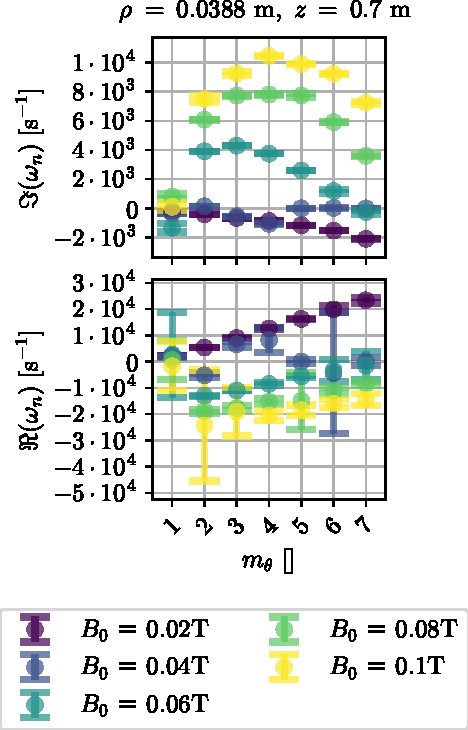
\includegraphics{fig/results/growthRates/growthRatesB0ModeNr}
        \label{fig:grBModeNr}
        \caption{$B$-dependency on the growth rates and angular velocities.
            Obtained from the simulations.}
\end{figure}
%
One can from \cref{fig:grBModeNr,fig:grAnalyticBModeNr} observe that the agreement between growth rate found in the simulation and growth rate found from the analytical expression is better for higher values of $B_0$.
It can also be observed that the angular frequency matches better for higher mode numbers, which is expected since the analytical expression was obtained from a slab geometry.

\section{Phase shift}
%
As explained in \ref{sec:simpleLin}, the instability requires a certain phase shift between $\phi$ and $n$ in order for the instability to occur.
Here, we will investigate how the phase shift varies with the $B$-field.

As shown in \cite{Pecseli2016book},
%
\begin{align}
    \Psi = \atan2\L(
    \Im\L[\frac{\om^*+ib\sigma_\|}{\om+ib\sigma_\|}\R],
    \Re\L[\frac{\om^*+ib\sigma_\|}{\om+ib\sigma_\|}\R]
    \R)
    \label{eq:analPhase}
\end{align}
%
gives us the phase shift between $n$ and $\phi$ for \cref{eq:analyticDisp}.

We would also like to find the phase-shift between $n$ and $\phi$ in the simulations.
The simplest way to do so is to extract one mode of the time signal Fourier transformed in time, and get the phase shift from finding the angle between the imaginary and real part for both $\phi$ and $n$.
However, as shown in \cref{fig:grB,fig:grBModeNr} the standard-deviation of the frequency can be quite high, which means that the frequency can change a lot during the linear phase.
The Hilbert transform could be used for finding the instantaneous phase-shift, but we will instead use a cross spectral density technique to give us the average phase-shift of the signals.

The cross spectral density can be found by first finding the cross correlation of the signals.
In the cross correlation the signals are first shifted with a time shift $\tau$ with respect to each other.
Excess parts of the signal will be padded with $0$s in order for the signals to have the same length.
The shifted signals are then multiplied and integrated over the time domain.
The cross correlation is then given by
%
\begin{align*}
    R_{n\phi}(\tau) = (n-\expt{n}_t) \star (\phi-\expt{\phi}_t),
\end{align*}
%
where $(a \star b)(\tau) \defined \defi{-\infty }{\infty}{a^{*}(t) b(t+\tau )}{t}$ denotes the cross correlation, and $a^*(t)$ denotes the complex conjugated.
Note that the time average has been subtracted from the signals in order for the zero padding in order to make sense.
The average time delay of the signals will therefore be the $\tau$ where the integral is the largest.
As noted in \cite{Huld1988}, a positive $R_{n\phi}$ corresponds to a positive particle flux.
In order to extract the phase-shift, we can Fourier transform $R_{n\phi}$ in order to get the cross spectrum density $S_{n\phi}$ .
As $S_{n\phi}$ is complex it can be written
%
\begin{align*}
    S_{n\phi}(f) = \mathcal{F}[R_{n\phi}(\tau)] = \L|S_{n\phi}(f)\R|\exp\L(i\Psi(f)\R),
\end{align*}
%
where $\mathcal{F}[R_{n\phi}(\tau)]$ denotes the Fourier transformed, and $\Psi$ is the phase angle between $n$ and $\phi$.
The dominating averaged phase shift will therefore be the $\Psi$ corresponding to the largest $\L|S_{n\phi}(f)\R|$, and can as usual be found by $\Psi = \atan2(\Im[S_{n\phi}], \Re[S_{n\phi}])$.

In this thesis we will use the periodogram to estimate the cross spectral density from the discrete time series of $n$ and $\phi$.
This corresponds to use a triangular window for the signals (see \cite{Miller2004book} for details).
The phase shifts from the simulations are shown in \cref{fig:phaseShift} together with the phase shifts found in \cref{eq:analyticDisp}.
%
\begin{figure}
    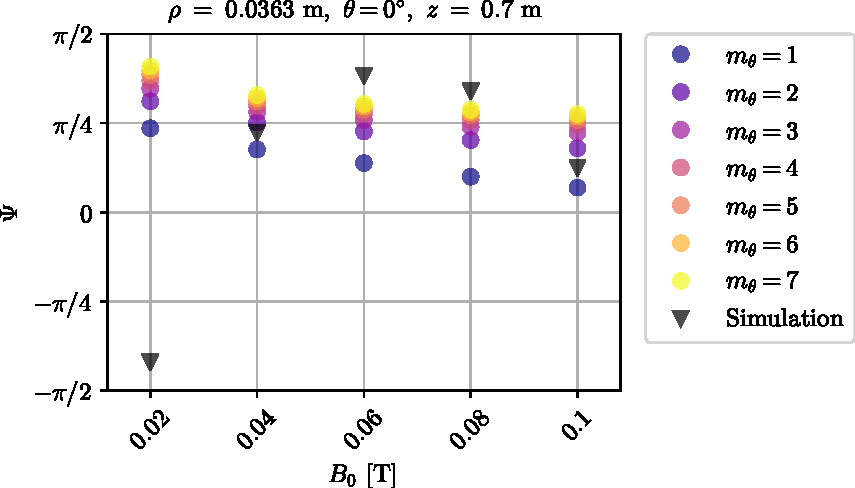
\includegraphics{fig/results/growthRates/phaseShift}
    \caption{
        Phase shift as a function of $B$.
        The different modes are calculated from \cref{eq:analPhase}, whereas the "Simulation" is the phase shift extracted from the simulations.
    }
    \label{fig:phaseShift}
\end{figure}
%
We note that a positive $\Psi$ is equivalent to a growth of the instability \cite{Garcia2001a}, and a negative $\Psi$ corresponds to a damping of the modes.
Apart from $B=0.02\T$ which were damped for all modes in the simulations, but had a small growth in the analytic expression, there are qualitatively good match between the phase shifts in \cref{fig:phaseShift}.

\section{Conclusion of the findings in the linear phase}
%
We will now summarize our findings in the linear phase and draw some conclusions from this.
In order to distinguish the drift wave instability from for example the Kelvin Helmholtz instability (which shares many of the same characteristics with the drift wave instability), the points in the following list must be fulfilled \cite{Jassby1972,Hendel1968}:
%
\begin{enumerate}[noitemsep]
    \item $\wt{n}/n$ peaks approximately at the position of the absolute maximum of the density.
    \item The perturbation has a finite parallel extension, typically in the order of the machine length.
    \item The perturbations are propagating in the electron diamagnetic drift direction.
    \item The density leads the potential.
\end{enumerate}
%
From \cref{fig:modeRotation,fig:dominatingMode} we can observe that point 1 is fulfilled.
These figures also indicate that point 2 is fulfilled.
Point 3 is fulfilled, with exception for $B_0=0.02\T$, as shown in \cref{fig:modeRotation,fig:grB,fig:grBModeNr}.
Finally, one can observe that point 4 is observed in \cref{fig:phaseShift}.

From this we conclude that the instability under investigation most probably is a drift wave instability.
The same conclusion has been reached for in VINETA in \cite{Schroder2005}.
